% Chapter Template

\chapter{Performance and Transferability of DeepBM: A Study with Syndiotactic Polystyrene} % Main chapter title
\label{bm_ps} % Change X to a consecutive number; for referencing this chapter elsewhere, use \ref{ChapterX}

In this chapter, DBM is applied to a challenging condensed-phase molecular system: syndiotactic polystyrene (sPS). The performance of DBM is analyzed in terms of three important aspects: 1) The general reverse-mapping capability of the model, i.e. the ability to reproduce a reference atomistic distribution from coarse-grained configurations. 2) The transferability of the model across different state points. To this end, DBM is trained solely on data obtained in a high-temperature melt and the model's transferability to lower temperatures is probed. 3) The transferability of DBM across chemical space. Here, DBM is trained on liquids of small molecules. After training, the model is deployed on the more challenging polymeric system of sPS. 

This chapter presents content that has been previously published in the following research articles. The content is reproduced here with kind permission from the other authors and the corresponding Journals published this work.

\hfill \break
\noindent \textit{Marc Stieffenhofer, Michael Wand, Tristan Bereau}\\
\textbf{Adversarial reverse mapping of equilibrated condensed-phase molecular structures}\\
Machine Learning: Science and Technology, Volume 1, Number 4\\
DOI: 10.1088/2632-2153/abb6d4\\
$\copyright$ IOP Publishing Ltd, 2020
\hfill \break

\noindent \textit{Marc Stieffenhofer, Tristan Bereau, Michael Wand}\\
\textbf{Adversarial reverse mapping of condensed-phase molecular structures: Chemical transferability}\\
APL Materials 9, Volume 9, Number 3\\
DOI: 10.1063/5.0039102\\
$\copyright$ AIP Publishing LLC, 2021
\hfill \break

\section{Set-up and Reference Data}

In this section, the reference data used to train and evaluate the performance of DBM is introduced. In addition, a baseline method is utilized to compare the backmapped results of DBM with a state-of-the-art method. 

\subsection{Syndiotactic Polystyrene}
\label{SEC:sPS}

\begin{figure}
  \centering
  \captionsetup{width=1.0\linewidth}
      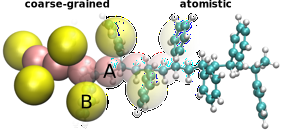
\includegraphics[width=0.70\textwidth]{./Figures/adversarial_backmapping/intro.pdf}
  \caption{Coarse-grained and atomistic representation of sPS. The coarse-grained monomer consists of two beads, denoted $A$ for the chain backbone and $B$ for the phenyl ring. \cite{stieffenhofer2020adversarial}}
  \label{FIG:sPS_single_chain}
\end{figure}

Polystyrene (PS) is an aromatic polymer made from the monomers styrene, which is an oragnic compound consisting entirely of carbon and hydrogen. Physical and chemical properties of PS depent significantly on its tacicity, i.e. the arrangement of the phenyl groups along the polymer backbone. In this study, syndiotactic polystyrene (sPS) is used, where the phenyl groups are arranged on alternating sides of the polymer backbone. An illustration of a single polymer chain with atomistic as well as coarse-grained resolution is shown in Fig. \ref{FIG:sPS_single_chain}. 

Despite its simple chemical structure, sPS displays a rich conformational space and exhibits complex polymorphic behavior. As such, sPS is a well suited candidate to study the transferability properties of DBM. Upon thermal annealing, a sPS melt undergoes a phase transition from amorphous to a crystalline phase at $T \approx 450$ K.\cite{liu2018polymorphism} Five different crystalline forms of sPS have been reported experimentally. Here, the focus is set on the $\alpha$ and $\beta$ polymorphs, which are illustrated in Fig. \ref{FIG:sPS_polymorphs}.

The atomistic data in this study is reported in Liu \emph{et al.};\cite{liu2018polymorphism} the underlying force field is based on the work of Mueller-Plathe.\cite{muller1996local} The system is sampled using Replica Exchange MD simulations, which are performed using the molecular dynamics package {\sc GROMACS} 4.6.\cite{hess2008gromacs} The simulations are carried out in the NPT ensemble using the velocity rescaling thermostat and the Parrinello-Rahman barostat. An integration timestep of $1$ fs is used. For additional details regarding the simulations the reader is referred to the work of Liu \emph{et al.}\cite{liu2018polymorphism}

Pairs of corresponding fine- and coarse-grained snapshots are generated starting from atomistic configurations, which are mapped onto the coarse-grained resolution. Three data sets are constructed from uncorrelated snapshots selected from different trajectories simulated at $T = 313$ K, $453$ K, and $568$ K. To cover a wide range of conformational space, each atomistic simulation was initialized from a different structure: The simulation at $313$ K started from a $\beta$ structure, at $453$ K from an $\alpha$ structure and at $568$ K from an amorphous configuration. The system includes $36$ polystyrene chains and each chain consists of $10$ monomers. Each data set contains $12$ snapshots fo rtrainng and $78$ snapshots for testing.

The fine-to-coarse mapping is based on the coarse-grained model developed by Fritz \emph{et al.}.\cite{fritz2009coarse} Each monomer is mapped onto two beads of different types, denoted $A$ for the chain backbone and $B$ for the phenyl ring (see Fig. \ref{FIG:sPS_single_chain}). Bonds are formed only between backbone and phenyl ring beads $A$-$B$, i.e. the coarse-grained polymer is represented as a linear chain. The coarse grained model, parameterized in the melt, is transferable to the crystalline phase and stabilizes the experimentally observed $\alpha$ and $\beta$ polymorphs. 

%In isotactic PS the phenyl groups are positioned on the same side of the polymer chain, while in syndiotactic PS the phenyl groups are arranged on alternating sides of the chain. In atactic PS the phenyl groups are arranged randomly. 

\subsection{Baseline method}

The results of DBM are compared with a generic backmapping scheme as described in Sec. \ref{SEC:bm_generic}. Specifically, the backmapping script developed by Wassenaar \emph{et al.} is utilized.\cite{wassenaar2014going} In a first step, this method places each particle on the weighted average position of the coarse-grained beads it corresponds to and optionally adds a random displacement. In addition, the protocol allows to apply geometric modifiers setting the alignment of the next particle cis, trans, out, or chiral with respect to the other particles. The modifiers are crucial for the performance of this method and require a careful construction by the user.

After the initial structure is generated, the protocol by Waasenaar \emph{et al.} continues with multiple cycles of force-field based energy minimization for relaxation. Here, the first cycle consists of $200$ steps and is performed without non-bonded interactions. Afterwards, all interactions are turned on and energy minimization continues with a total number of $5000$ steps. The original protocol continues with several cycles of position restrained MD simulations to equilibrate the relaxed system. However, comparing DBM with such equilibrated structures is pointless as they would obviously reproduce the correct Boltzmann distribution. DBM aims at generating molecular structures without relying on further MD simulations. Therefore, the script by Waasenaar \emph{et al.} is stopped after the relaxation,to allow for a more stringent comparison.

\section{General Performance}
\label{SEC:DBM_general_performance}

At first, the general performance of DBM is probed. To this end, DBM is trained on the high-temperature, amorphous data set at $568$ K. After training, the model is deployed to test data, i.e. hold-out data at the same temperature.   

\subsection{Results}

\begin{figure}
  \centering
  \captionsetup{width=1.0\linewidth}
      \includegraphics[width=1.05\textwidth]{./Figures/adversarial_backmapping/sPS_temp_trans/ff_dists_and_rdf.pdf}
  \caption{ Canonical distributions for various force-field interaction terms at (left) $T$ = 568 K, (middle) $T$ = 453 K and (right) $T$ = 313 K for reference structures (black), structures generated with the baseline, energy-minimization-based backmapping method (red), and the new method DBM (blue). The model is trained solely on the high temperature data (left), but deployed at lower temperatures (middle and right). (a)–(c) C-C-C backbone angle, (d)–(f) C-C-C-C backbone dihedral, (g)–(i) C-C-C-C improper dihedral, (j)–(l) Lennard-Jones energies, and (m)–(o) radial distribution functions, g(r), of the non-bonded carbon atoms.\cite{stieffenhofer2020adversarial}}
  \label{FIG:sPS_temp_trans_ff_dists}
\end{figure}

Fig. \ref{FIG:sPS_temp_trans_ff_dists} displays distribution functions for several structural and energetic properties of sPS. The distributions of intramolecular carbon backbone angle and dihedral, shown in FIG. \ref{FIG:sPS_temp_trans_ff_dists} (a) and (d), are in excellent agreement with the reference distributions. On the other hand, structures generated with the baseline method show too narrow distributions, which is expectable from an approach based on energy minimization. As shown in Fig. \ref{FIG:sPS_temp_trans_ff_dists} (g), the distribution for the carbon improper dihedral of the phenyl group is slightly too narrow for configruations generated with DBM. However, the small range of angles due to the imposed planarity of the ring has to be emphazied. The distribution of the baseline method is even more peaked, i.e. fluctuations around the planar structure are significantly suppressed.

A very important aspect towards generating well-equilibrated configurations in a condensed environment is the correct reproduction of Lennard-Jones energies. Fig. \ref{FIG:sPS_temp_trans_ff_dists} (j) displays the distribution of Lennard-Jones energies obtained for each chain separately. While structures generated with DBM show slightly too large high-energy tails, the overall match with the reference distribution is remarkably well. On the other hand, the baseline method systematically and drastically over-stabilizes the system. 

Further, the radial distribution function is analyzed to probe the ability of DBM to reproduce large-scale structural features. Fig. \ref{FIG:sPS_temp_trans_ff_dists} (m) displays the pair correlation function $g(r)$ for non-bonded carbon pairs. Structures generated with DBM show an excellent agreement with the reference distribution indicating that the local packing of the polymer chains is well reproduced. The baseline method is not able to reproduce the pair correlation correctly.

\subsection{Discussion}

DBM is an ML approach for the backmapping of coarse-grained molecular structures. The DNN based model learns to reproduce local features guided by large-scale structures from a coarse-grained snapshot. Here, it is applied to the high-temperature data set of an complex condensed-phase molecular system made of sPS chains. The results are compared with a baseline method based on energy-minimization.

It is shown that he method reproduces structural and energetic properties of the reference system remarkably well. DBM yields well-equilibrated configurations of a Boltzmann distribution at a state point it was trained on. On the other hand, the baseline method based on energy minimization over stabilizes the system. As such, it does not account for the diversity of microstates at a specific canonical state point. Consequently, further MD simulations controlled by a thermostat are required to recover the correct state point.

\section{Temperature Transferability: From Melt to Crystal}

After successfully recovering the state point DBM was trained on, the model's ability to transfer across temperatures is probed. As illustrated in Fig. \ref{FIG:sPS_polymorphs}, the training of DBM is fixed to the high-temperature ensemble but testing is performed at lower temperatures \textit{without} reparametrization. Specifically, the model is trained at $568$ K and tested at $453$ K and $313$ K. Importantly, the sPS system undergoes a phase transition at $\approx 450$ K, going from an amorphous phase to a crystalline state with different polymorphs. As such, the test data sets not only differ in terms of temperature compared to the training data set, but also display different state points, i.e. the $\alpha$ and $\beta$ polymorphs. 

\begin{figure}
  \centering
      \includegraphics[width=0.6\textwidth]{./Figures/adversarial_backmapping/sPS_temp_trans/ps_polymorphs.pdf}
  \caption{Polymorphism of Polystyrene. At high temperature ($T$ = 568 K) the system stabilizes an amorphous phase. At lower temperatures the CG model mostly stabilizes the $\alpha$ polymorph at $T$ = 453 K and the $\beta$ polymorph at $T$ = 313 K. DeepBackmap is trained solely on the high-temperature ensemble ($T$ = 568 K) and test its transferability to the lower temperatures. \cite{stieffenhofer2020adversarial}}
  \label{FIG:sPS_polymorphs}
\end{figure}

\subsection{Results}

As shown in Fig. \ref{FIG:sPS_temp_trans_ff_dists} (middle and right culumn), the distributions of structural and energetic features display a number of significant changes upon cooling: distributions of angles become narrower, the side peak in the backbone dihedral vanishes, the distributions of Lennard-Jones energies are shifted towards lower energies and the pair correlation of non-bonded carbon atoms is more peaked. 

\subsubsection{Distributions of Structural and Energetic Features}

DBM adapts remarkbly well to the crystalline state points. Fig. \ref{FIG:sPS_temp_trans_ff_dists} (b,c,e,f,h,i) indicate that the angle and dihedral distributions for structures generated with DBM follow the reference distributions and become narrower. Lennard-Jones energies displayed in Fig. \ref{FIG:sPS_temp_trans_ff_dists} (k,l) are also shifted and match with the reference distributions. Moreover, the local packing of the sPS chains is perfectly reproduced even in the crystalline phase, as indicated in Fig. \ref{FIG:sPS_temp_trans_ff_dists} (n,o). 

On the other hand, the baseline method does not adapt well to lower temperatures. The method based on energy minimization is not able to generate the correct features at the crystalline state points, but retains much of its features found at high temperature. This becomes especially apparent for the side peak of the backbone dihedral and the flat pair correlation function $g(r)$.

\subsubsection{Sketch-Map}

\begin{figure}
  \centering
      \includegraphics[width=1.1\textwidth]{./Figures/adversarial_backmapping/sPS_temp_trans/sm_snapshots.pdf}
  \caption{ Low-dimensional structural space of condensed-phase configurations at (a) $T$ = 568 K, (b) $T$ = 453K and (c) $T$ = 313 K. For each panel, snapshots are backmapped from identical coarse-grained configurations, highlighting the overlap between reference and DeepBackmap, but disconnect from the baseline method.\cite{stieffenhofer2020adversarial}}
  \label{FIG:sPS_temp_trans_SM}
\end{figure}

Evaluating large-scale structural features beyond pair-statistics is challenging, since the high dimensionality of the system does not allow to directly visualize the configuration space. For this reason, dimensionality reduction is applied to further examine the model's accuracy at higher order. As explained in Sec. \ref{SEC:ML_latent_variables}, linear dimensionality reduction techniques are insufficient in many cases to capture the global structure of data obtained from MD trajectories. Therefore, Sketch-Map (SM) is applied to build a two-dimensional map representing proximity relationships between sPS chains. 

The descriptors for the sPS chains consist of a set of representations of the local environments $\mathcal{H}$ centered around alternating backbone carbon atoms that are directly linked to a phenyl group. The pairwise distance between two such environments is encoded using a similarity kernel $k(\mathcal{H}, \mathcal{H}') = \mathbf{p}(\mathcal{H}) \mathbf{p}(\mathcal{H'})$ based on the normalized many-body smooth overlap of atomic position (SOAP) representation $\mathbf{p}(\mathcal{H})$.\cite{} Hydrogen atoms are neglected in the SOAP representation. To compare two sPS chains $a$ and $b$, the covariance matrix 

\begin{equation}
 C_{ij}(a,b) = \mathbf{p}(\mathcal{H}^a_i) \mathbf{p}(\mathcal{H}^b_j)
\end{equation}

is computed, which contains the complete information of the pairwise similarity of all local environments taken into account between the two structures. In order to obtain a global similarity kernel $k(a,b)$, the covariance matrix $C_{ij}(a,b)$ has to be mapped to a single scalar value, which is achieved using a regularized entropy match kernel.\cite{}

Fig. \ref{FIG:sPS_temp_trans_SM} displays the obtained two-dimensional map, where each point represents a single sPS polymer chain. A number of clusters is shown that correspond to different environments. The reference data (black) shows a single cluster for the low-temperature data at $313$ K (Fig. \ref{FIG:sPS_temp_trans_SM} (c)) corresponding to the $\beta$ polymorph. The high-temperature data at $568$ K (Fig. \ref{FIG:sPS_temp_trans_SM} (a)) is mapped to multiple clusters indicating more diversity, i.e. it includes amorphous, $\alpha$ and other structures. The data set at an intermediate temperature $453$ K (Fig. \ref{FIG:sPS_temp_trans_SM} (b)) shows less diversity and is mapped mostly to the cluster corresponding to the $\alpha$ polymorph, but still contains some amorphous and other structures.

Structures obtained with DBM (blue) overlap significantly with the reference points for all three data sets indicating closeness in configuration space and high fidelity of the backmapped structures. This is in strong contrast to the energy-minimized structures obtained with the baseline method, which cover different areas in the two-dimensional projection of configuration space. Moreover, the baseline method fails to recover the correct number of clusters for all three temperatures highlighting a lack of temperature sensitivity.

\subsubsection{MD Simulation}

\subsection{Discussion}

In this section, the temperature transferability of DBM is probed. While training of the model is fixed to melt configurations at high temperature, it is deployed at lower temperatures, where the sPS system is in a crystalline state. However, DBM retains its performance displayed in Sec. \ref{SEC:DBM_general_performance} and reproduces the reference distributions with remarkable accuracy. In addition, a higher-order investigation, facilitated by the Sketchmap algorithm, emphasizes the high structural fidelity. As such, the model learns to reproduce local correlations that are transferable across different state points. This is in strong contrast to the baseline method, which lacks accuracy and temperature sensitivity. 

These remarkable transferability features of DBM can be rationalized in terms of a scale-separation: The model learns to reproduce well-equilibrated local correlations while large-scale features are dictated by the coarse-grained snapshot. As such, the backmapped structure is composed of two sources of information, i.e. 1) the learned local features and 2) the coarse-grained structure. However, most of the temperature dependence is carried by the latter, as it is shown by Liu et al. that the applied coarse-grained model reproduces the crystallization transition remarkably well. On the other hand, local features are less temperature sensitive, since they correspond primarily to covalent interactions that operate on energy scales significantly larger than $k_B T$. As such, the local correlations learned in the melt are transferable across a phase transition. However, it is not clear wheather the other direction, i.e. training at low temperature and transferring to higher temperatures, would yield satisfactory results, because of the broader conformational space spanned at higher temperatures.

\section{Chemical Transferability: From Small Molecules to Polymers}



\subsection{Results}

\begin{figure}
  \centering
  \captionsetup{width=1.0\linewidth}
      \includegraphics[width=1.05\textwidth]{./Figures/adversarial_backmapping/sPS_chem_trans/angles.pdf}
  \caption{ \cite{stieffenhofer2020adversarial}}
  \label{fig_bm_intro}
\end{figure}

\begin{figure}
  \centering
  \captionsetup{width=1.0\linewidth}
      \includegraphics[width=1.05\textwidth]{./Figures/adversarial_backmapping/sPS_chem_trans/dihs.pdf}
  \caption{ \cite{stieffenhofer2020adversarial}}
  \label{fig_bm_intro}
\end{figure}

\begin{figure}
  \centering
  \captionsetup{width=1.0\linewidth}
      \includegraphics[width=1.05\textwidth]{./Figures/adversarial_backmapping/sPS_chem_trans/non_bonded.pdf}
  \caption{ \cite{stieffenhofer2020adversarial}}
  \label{fig_bm_intro}
\end{figure}


\begin{figure}
  \centering
  \captionsetup{width=1.0\linewidth}
      \includegraphics[width=1.05\textwidth]{./Figures/adversarial_backmapping/sPS_chem_trans/sm_ref_p1.pdf}
  \caption{ \cite{stieffenhofer2020adversarial}}
  \label{fig_bm_intro}
\end{figure}

\begin{figure}
\hspace*{-1cm}
  \centering
  \captionsetup{width=1.0\linewidth}
      \includegraphics[width=1.2\textwidth]{./Figures/adversarial_backmapping/sPS_chem_trans/hm.pdf}
  \caption{ \cite{stieffenhofer2020adversarial}}
  \label{fig_bm_intro}
\end{figure}
\subsection{Discussion}
